% Options for packages loaded elsewhere
\PassOptionsToPackage{unicode}{hyperref}
\PassOptionsToPackage{hyphens}{url}
%
\documentclass[
  10pt,
]{article}
\usepackage{lmodern}
\usepackage{amssymb,amsmath}
\usepackage{ifxetex,ifluatex}
\ifnum 0\ifxetex 1\fi\ifluatex 1\fi=0 % if pdftex
  \usepackage[T1]{fontenc}
  \usepackage[utf8]{inputenc}
  \usepackage{textcomp} % provide euro and other symbols
\else % if luatex or xetex
  \usepackage{unicode-math}
  \defaultfontfeatures{Scale=MatchLowercase}
  \defaultfontfeatures[\rmfamily]{Ligatures=TeX,Scale=1}
  \setmainfont[]{Verdana}
  \setsansfont[]{Verdana}
  \setmonofont[]{Verdana}
\fi
% Use upquote if available, for straight quotes in verbatim environments
\IfFileExists{upquote.sty}{\usepackage{upquote}}{}
\IfFileExists{microtype.sty}{% use microtype if available
  \usepackage[]{microtype}
  \UseMicrotypeSet[protrusion]{basicmath} % disable protrusion for tt fonts
}{}
\makeatletter
\@ifundefined{KOMAClassName}{% if non-KOMA class
  \IfFileExists{parskip.sty}{%
    \usepackage{parskip}
  }{% else
    \setlength{\parindent}{0pt}
    \setlength{\parskip}{6pt plus 2pt minus 1pt}}
}{% if KOMA class
  \KOMAoptions{parskip=half}}
\makeatother
\usepackage{xcolor}
\IfFileExists{xurl.sty}{\usepackage{xurl}}{} % add URL line breaks if available
\IfFileExists{bookmark.sty}{\usepackage{bookmark}}{\usepackage{hyperref}}
\hypersetup{
  pdftitle={Wellbeing Survey Report},
  hidelinks,
  pdfcreator={LaTeX via pandoc}}
\urlstyle{same} % disable monospaced font for URLs
\usepackage[left = 2cm, right = 2cm, top = 2cm, bottom = 2cm]{geometry}
\usepackage{graphicx,grffile}
\makeatletter
\def\maxwidth{\ifdim\Gin@nat@width>\linewidth\linewidth\else\Gin@nat@width\fi}
\def\maxheight{\ifdim\Gin@nat@height>\textheight\textheight\else\Gin@nat@height\fi}
\makeatother
% Scale images if necessary, so that they will not overflow the page
% margins by default, and it is still possible to overwrite the defaults
% using explicit options in \includegraphics[width, height, ...]{}
\setkeys{Gin}{width=\maxwidth,height=\maxheight,keepaspectratio}
% Set default figure placement to htbp
\makeatletter
\def\fps@figure{htbp}
\makeatother
\setlength{\emergencystretch}{3em} % prevent overfull lines
\providecommand{\tightlist}{%
  \setlength{\itemsep}{0pt}\setlength{\parskip}{0pt}}
\setcounter{secnumdepth}{-\maxdimen} % remove section numbering
\usepackage{booktabs}
\usepackage{longtable}
\usepackage{array}
\usepackage{multirow}
\usepackage{wrapfig}
\usepackage{float}
\usepackage{colortbl}
\usepackage{pdflscape}
\usepackage{tabu}
\usepackage{threeparttable}
\usepackage{threeparttablex}
\usepackage[normalem]{ulem}
\usepackage{makecell}
\usepackage{xcolor}

\title{Wellbeing Survey Report}
\author{}
\date{\vspace{-2.5em}28 January 2021}

\begin{document}
\maketitle

{
\setcounter{tocdepth}{3}
\tableofcontents
}
\newpage

\hypertarget{introduction}{%
\section{Introduction}\label{introduction}}

The wellbeing survey was created to capture how the data lab team were
feeling and how they were coping in and outside of the workplace. It
also provided the team an anonymous way to express any concerns or
suggestions directly to management and senior leadership teams.

The response rate has been relatively high each week and comments have
been provided which have been fed directly back to SLT.

Since the wellbeing survey started, more teams within NDEC have shown
interest in rolling the survey out to their own team members.

\hypertarget{responses}{%
\section{Responses}\label{responses}}

The survey was first sent out on 4/11/2020 and then on a weekly basis.
More people have been added to distribution list. The table below shows
how many people have responded to the survey each week.

\begin{table}[H]

\caption{\label{tab:responses}Count of responses per survey}
\centering
\fontsize{12}{14}\selectfont
\begin{tabular}[t]{|>{}l||>{}l|r}
\toprule
survey\_date & survey\_month & response\_n\\
\midrule
\cellcolor{gray!6}{2020-11-04} & \cellcolor{gray!6}{2020-11-01} & \cellcolor{gray!6}{13}\\
2020-11-11 & 2020-11-01 & 12\\
\cellcolor{gray!6}{2020-11-18} & \cellcolor{gray!6}{2020-11-01} & \cellcolor{gray!6}{10}\\
2020-11-24 & 2020-11-01 & 13\\
\cellcolor{gray!6}{2020-12-02} & \cellcolor{gray!6}{2020-12-01} & \cellcolor{gray!6}{12}\\
2020-12-09 & 2020-12-01 & 13\\
\cellcolor{gray!6}{2020-12-16} & \cellcolor{gray!6}{2020-12-01} & \cellcolor{gray!6}{12}\\
2020-12-22 & 2020-12-01 & 10\\
\cellcolor{gray!6}{2020-12-30} & \cellcolor{gray!6}{2020-12-01} & \cellcolor{gray!6}{5}\\
\bottomrule
\end{tabular}
\end{table}

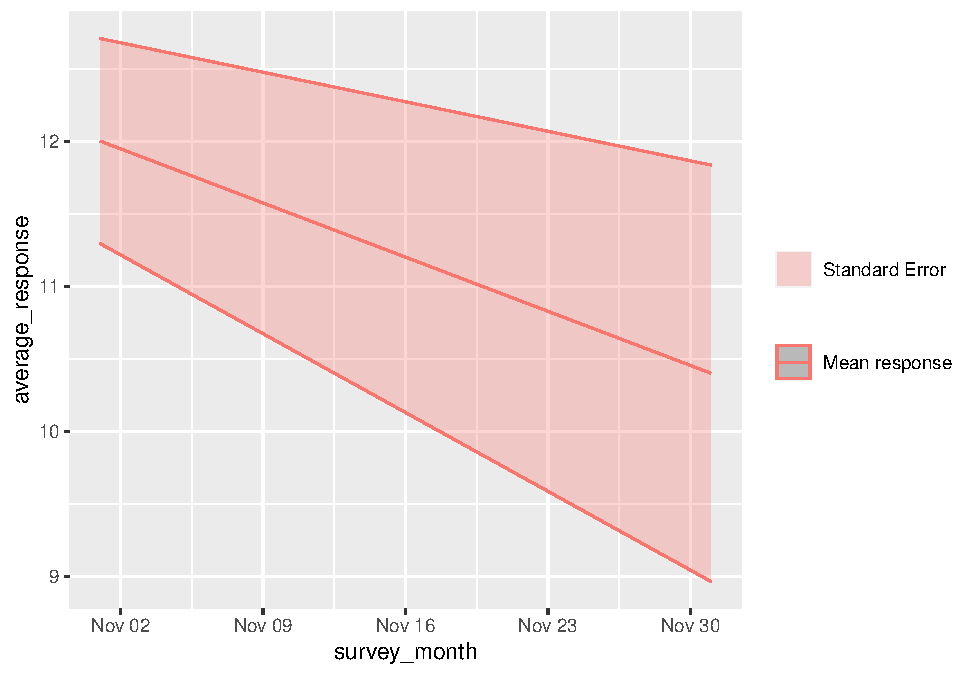
\includegraphics{../pdf/Report_files/figure-latex/monthly trend-1.pdf}

\hypertarget{plots}{%
\section{Plots}\label{plots}}

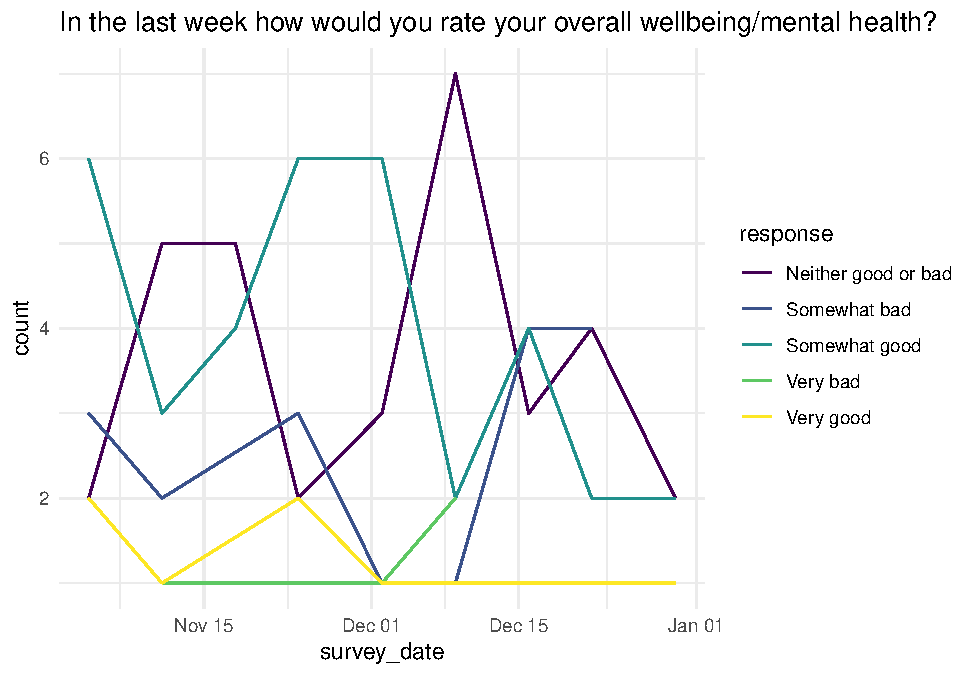
\includegraphics{../pdf/Report_files/figure-latex/plot_functions-1.pdf}
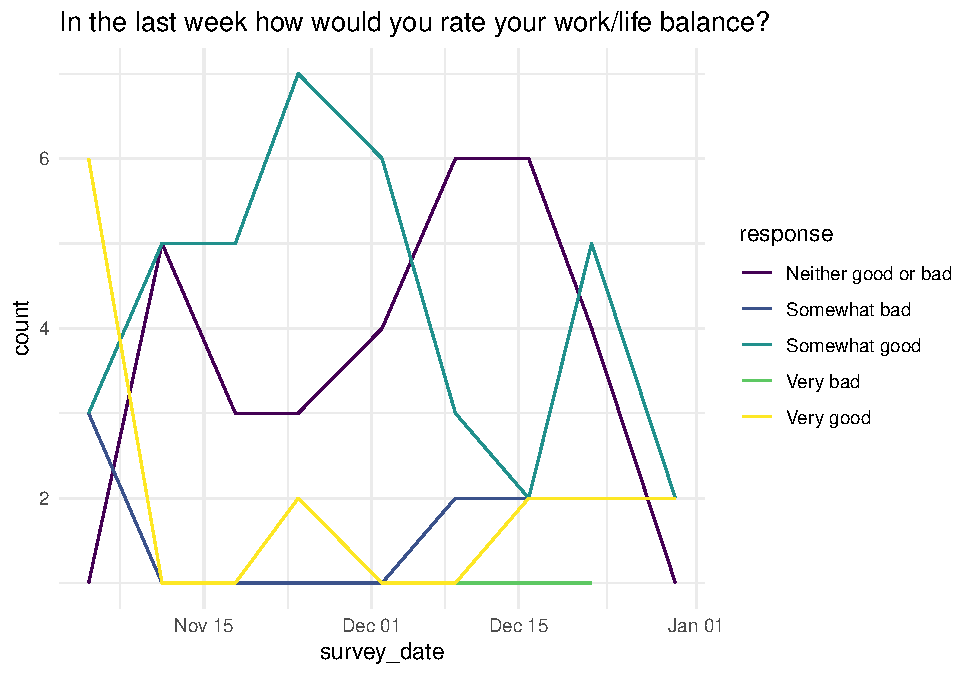
\includegraphics{../pdf/Report_files/figure-latex/plot_functions-2.pdf}
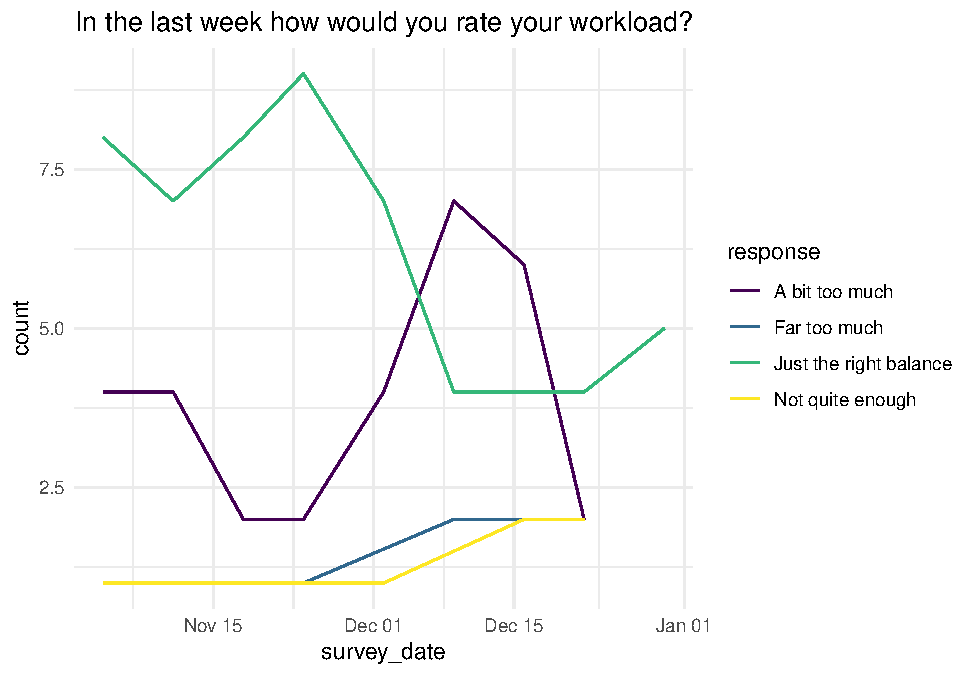
\includegraphics{../pdf/Report_files/figure-latex/plot_functions-3.pdf}
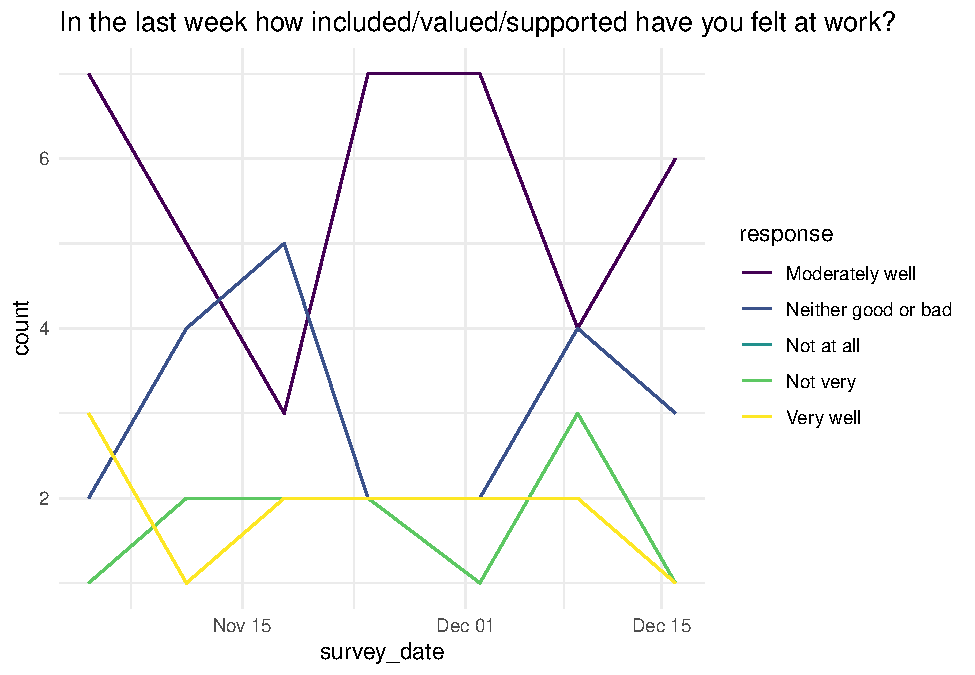
\includegraphics{../pdf/Report_files/figure-latex/plot_functions-4.pdf}
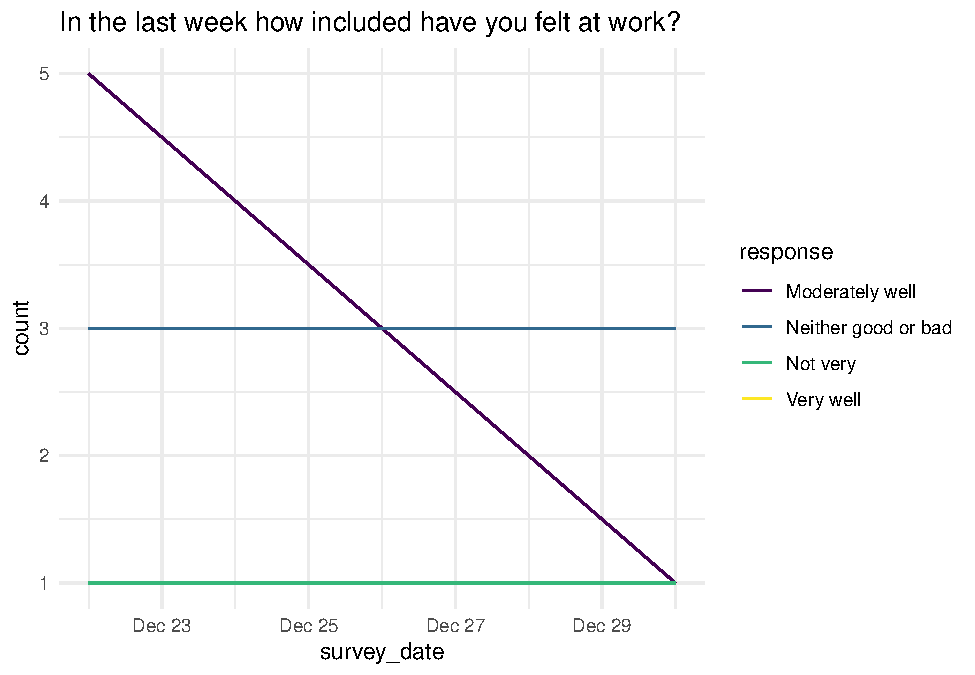
\includegraphics{../pdf/Report_files/figure-latex/plot_functions-5.pdf}
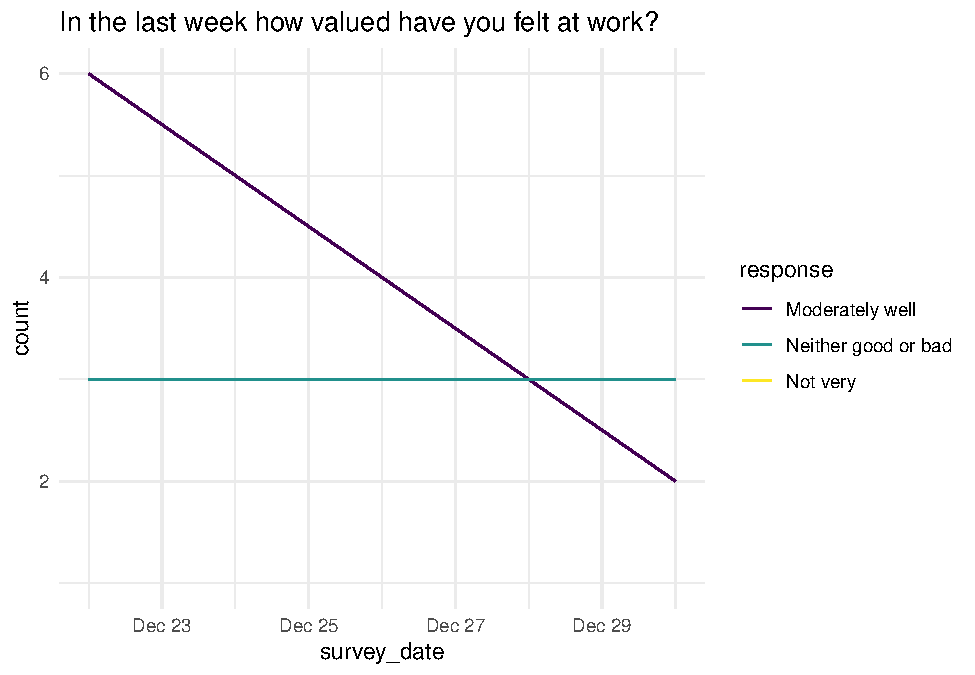
\includegraphics{../pdf/Report_files/figure-latex/plot_functions-6.pdf}
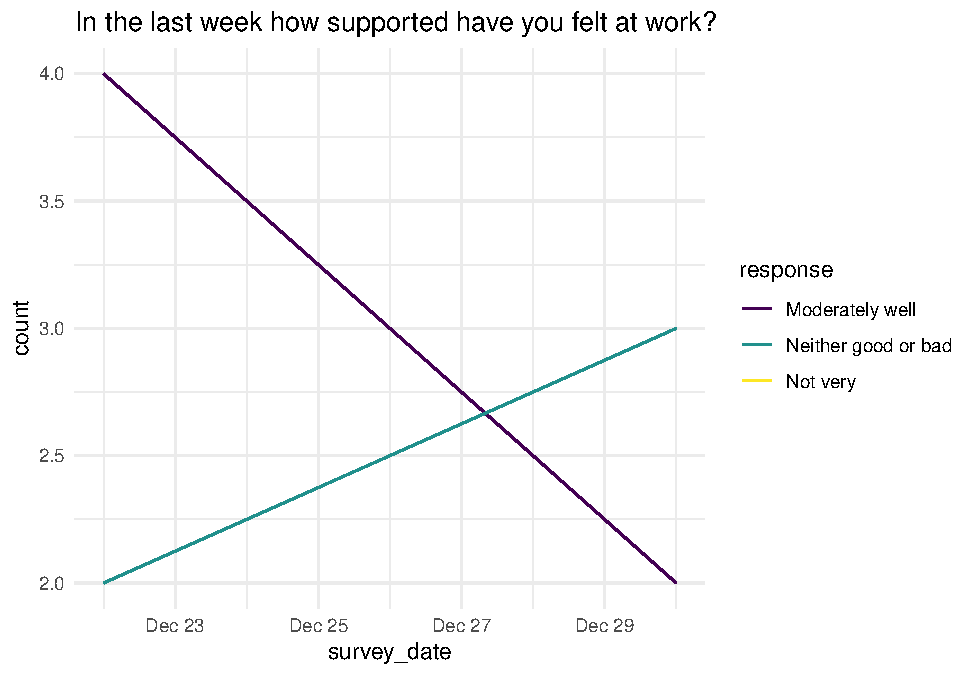
\includegraphics{../pdf/Report_files/figure-latex/plot_functions-7.pdf}
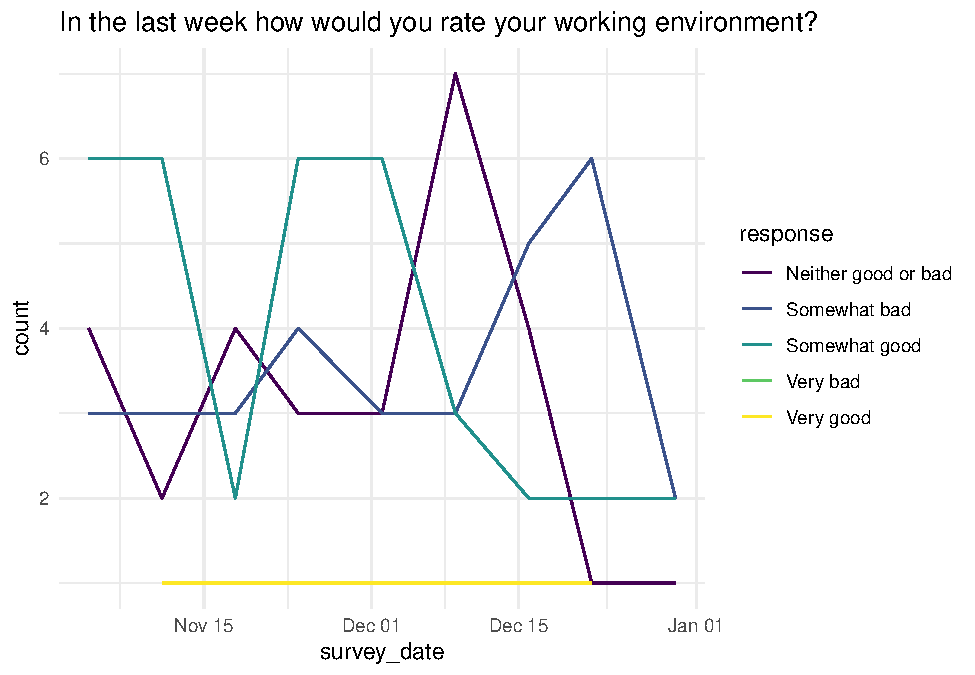
\includegraphics{../pdf/Report_files/figure-latex/plot_functions-8.pdf}
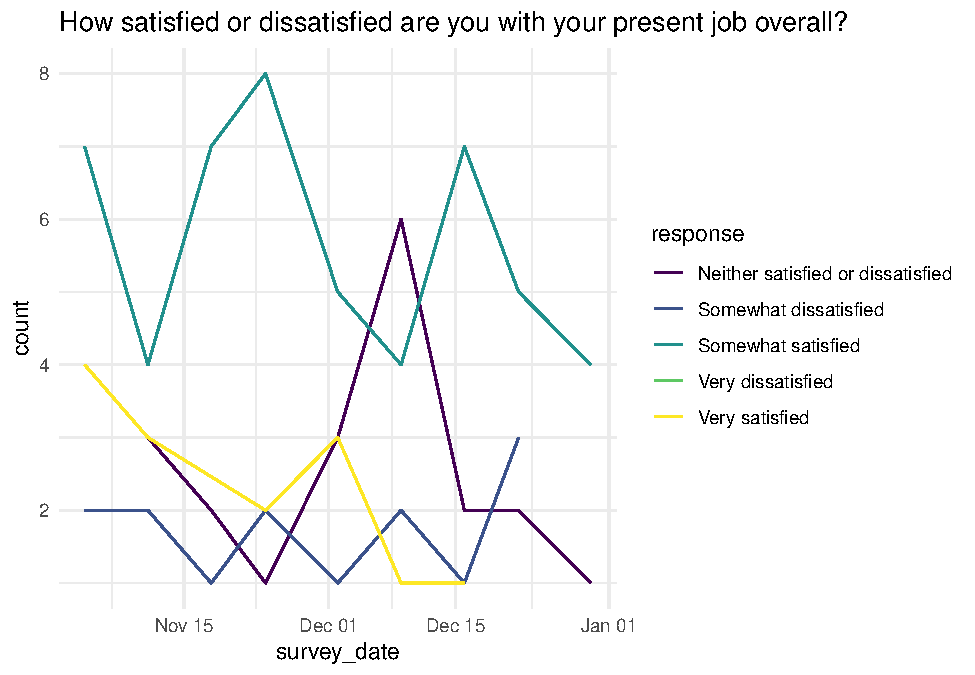
\includegraphics{../pdf/Report_files/figure-latex/plot_functions-9.pdf}

\hypertarget{score-over-time}{%
\section{Score over time}\label{score-over-time}}

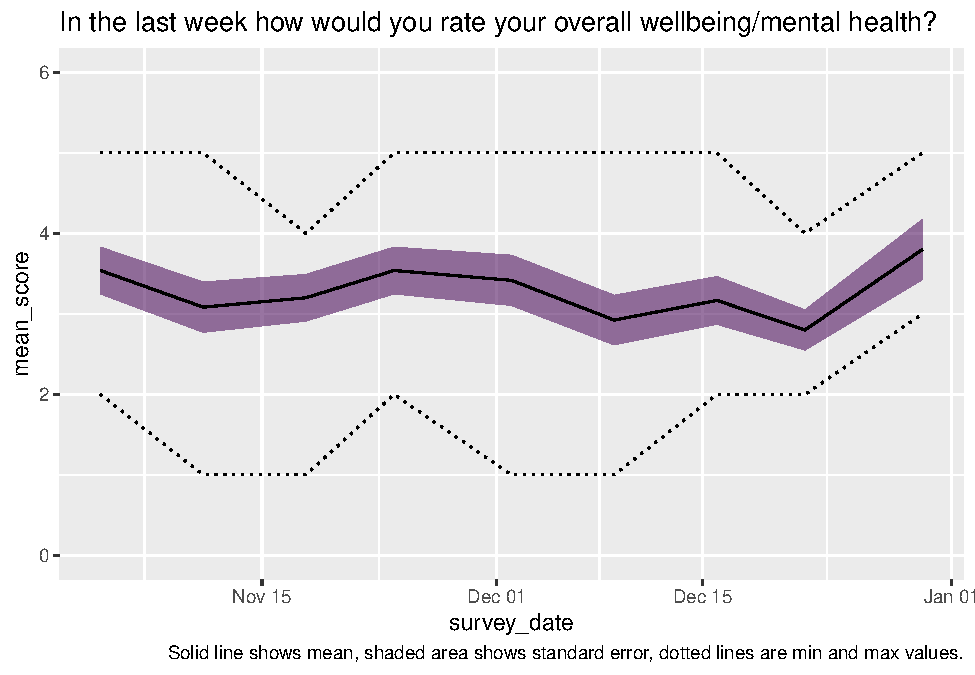
\includegraphics{../pdf/Report_files/figure-latex/likert-1.pdf}
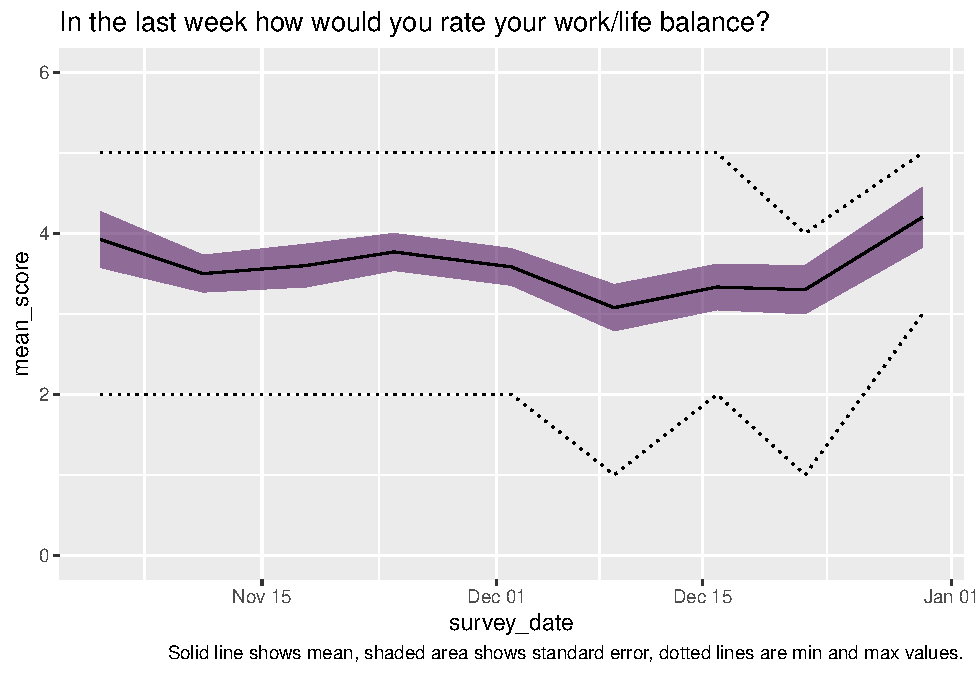
\includegraphics{../pdf/Report_files/figure-latex/likert-2.pdf}
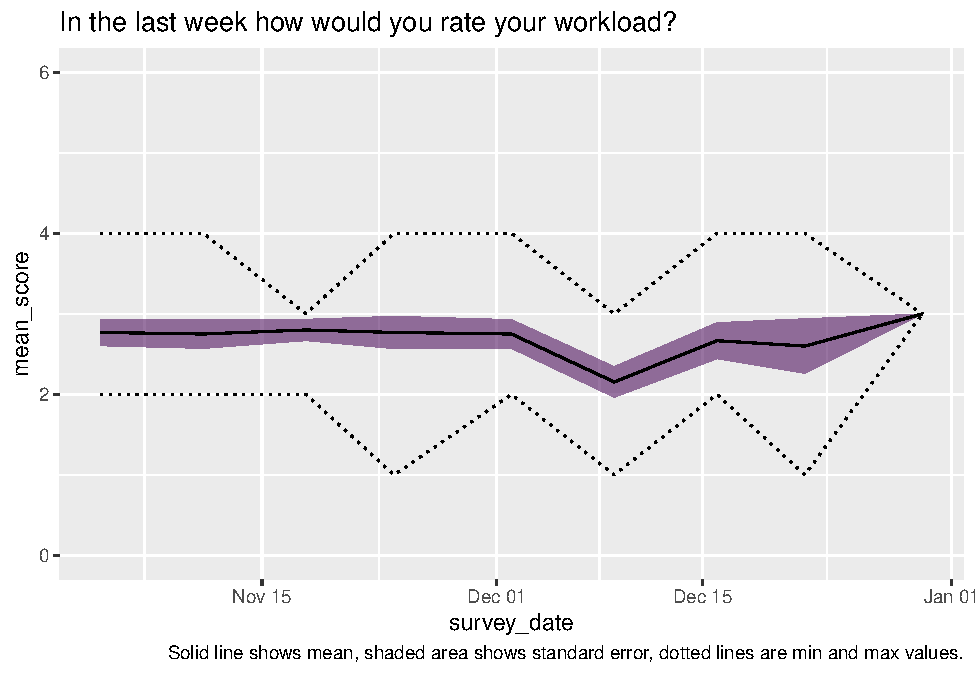
\includegraphics{../pdf/Report_files/figure-latex/likert-3.pdf}
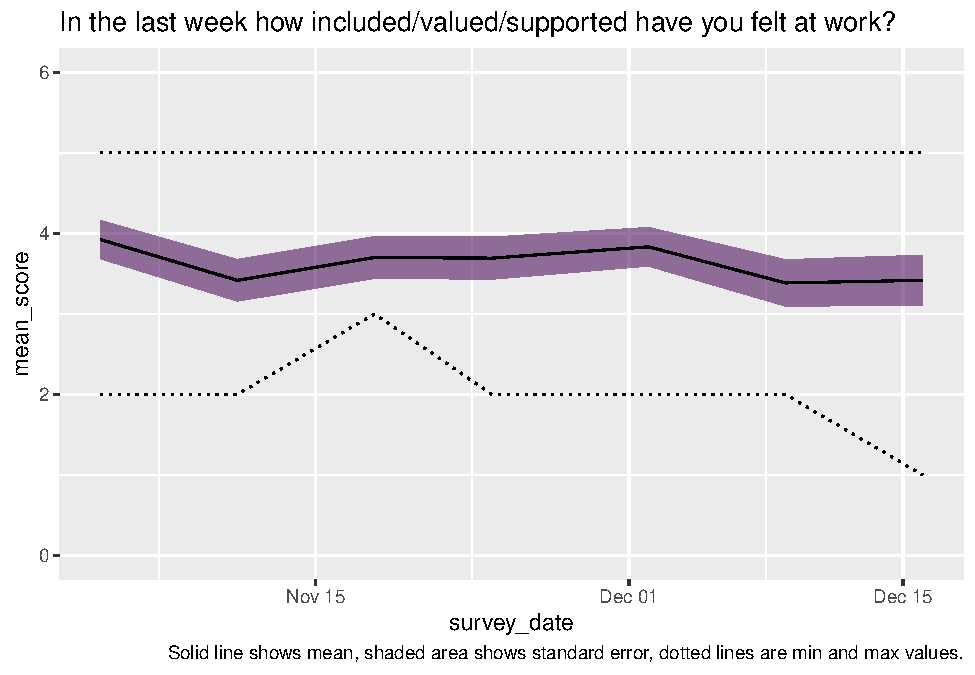
\includegraphics{../pdf/Report_files/figure-latex/likert-4.pdf}
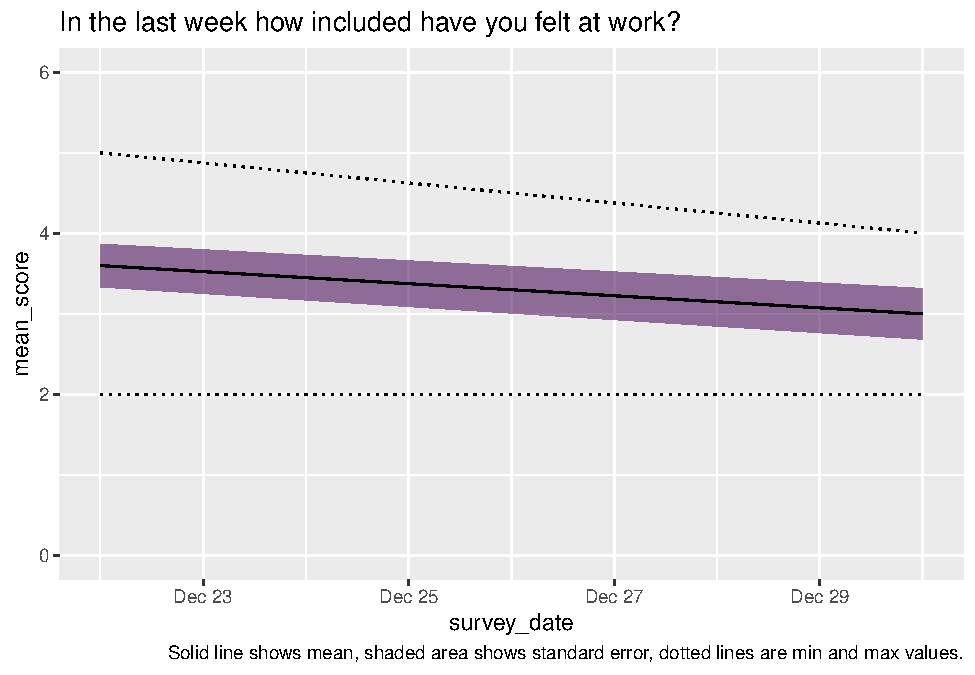
\includegraphics{../pdf/Report_files/figure-latex/likert-5.pdf}
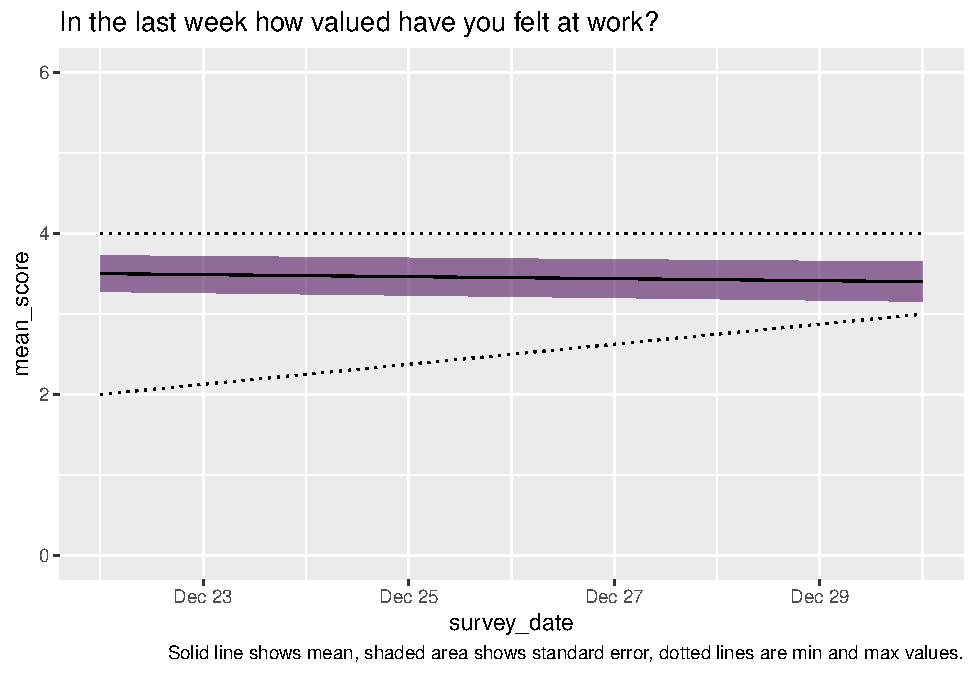
\includegraphics{../pdf/Report_files/figure-latex/likert-6.pdf}
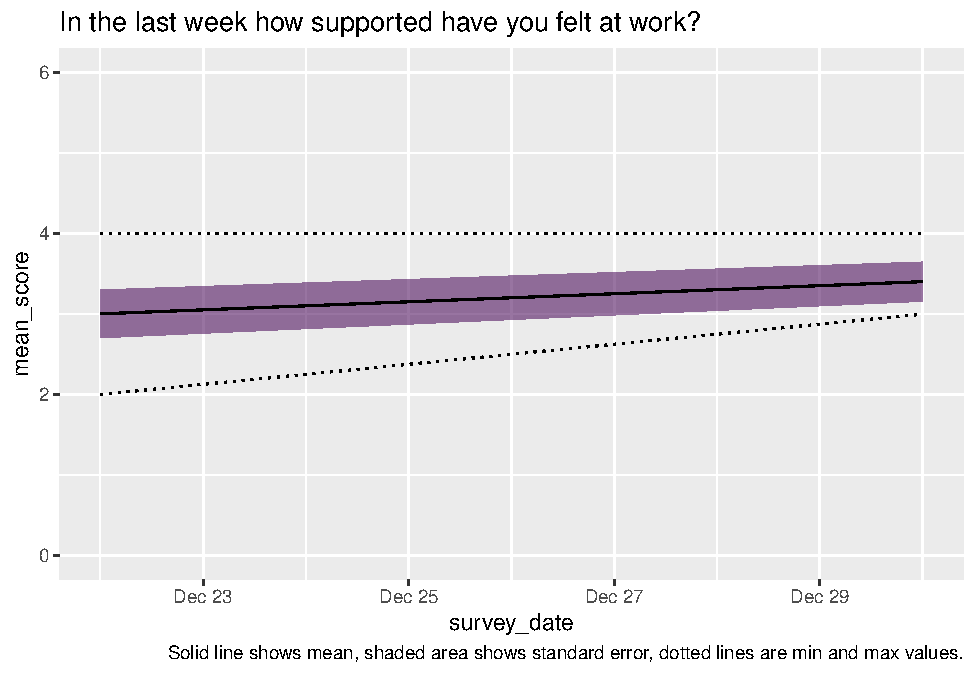
\includegraphics{../pdf/Report_files/figure-latex/likert-7.pdf}
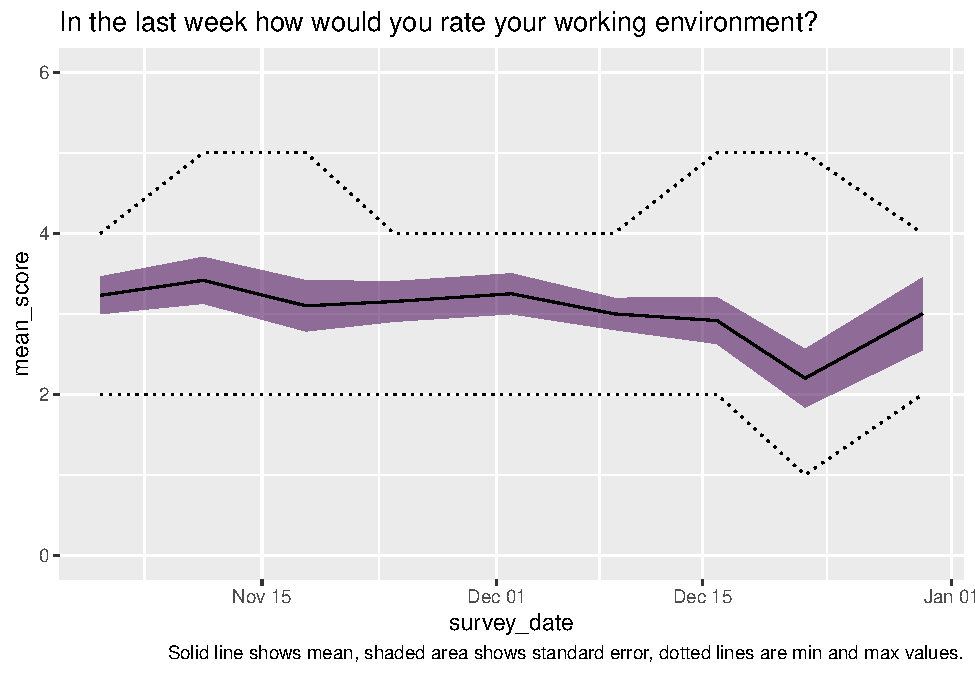
\includegraphics{../pdf/Report_files/figure-latex/likert-8.pdf}
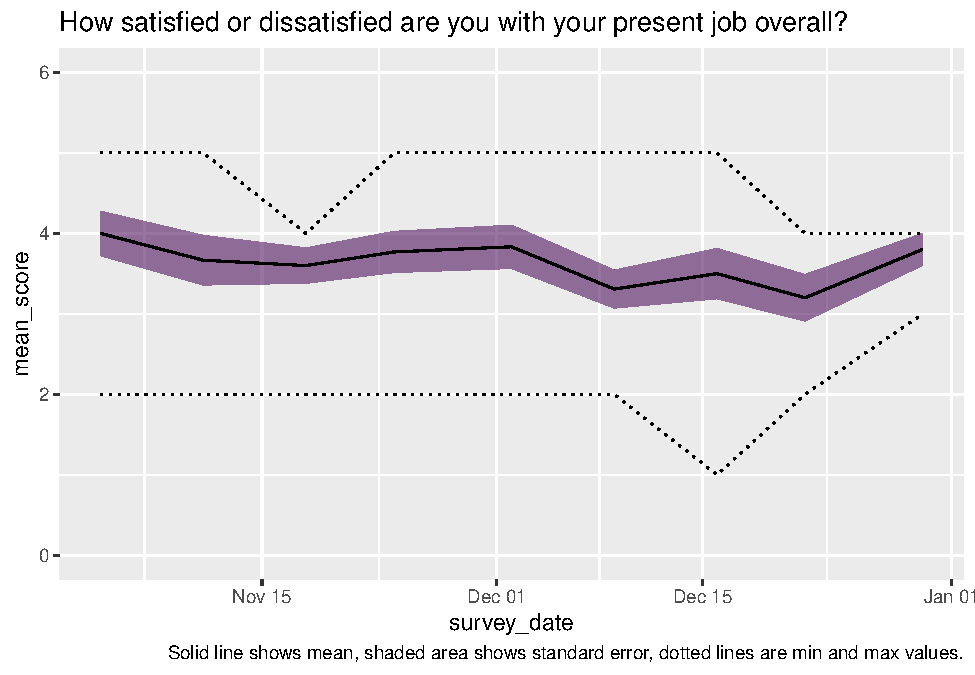
\includegraphics{../pdf/Report_files/figure-latex/likert-9.pdf}

\end{document}
